%Edit 0041 ZZZ to report number nnnn 
%Edit 3.1.4 YYMILE to milestone number m.m.m
%Edit Report on specification and integration of middle layer modules YYTITLE to report title - Words Start with Caps
\documentclass[11pt,twoside,a4paper]{article}
%%======================================================================
%% PACKAGES:
%%
%\usepackage{times}               % Times+Helvetica+Courier fonts
\usepackage{helvet}              % helvetica + cmr
\usepackage{fancyhdr}       % package for headers/footers
\usepackage{amsmath}
\usepackage{amssymb}
\usepackage{graphicx}            % Graphics.
%\usepackage{a4}                  % page layout to fit A4
%\usepackage{lastpage}            % get page no of last page
%\usepackage{ifthen}              % logical branching
\usepackage{hyperref}            %insert hyper-links
\usepackage{latexsym}
% uncomment the following to override auto page total
%\pptotal{20}
%%======================================================================

% ensure sans-serif font used throughout
\renewcommand{\familydefault}{\sfdefault}

\newcommand{\culhamissueno}{1.00}%<==edit
\newcommand{\culhamshorttitle}{CD/EXCALIBUR-FMS/0041}%<==edit
\newcommand{\Sec}[1]{Section~\ref{sec:#1}}
\newcommand{\Fig}[1]{Figure~\ref{fig:#1}}
\newcommand{\Tab}[1]{Table~\ref{tab:#1}}
\newcommand{\Eq}[1]{Equation~(\ref{eq:#1})}
\newcommand{\Eqs}[2]{Equations(\ref{eq:#1}) and~(\ref{eq:#2})}
\newcommand{\Figs}[2]{Figures~\ref{fig:#1}--~\ref{fig:#2}}
%Bold lc for script names, tt for computer code and file-names
%\F{NEPTUNE} always in caps
\newcommand{\F}[1]{\textsc{#1}}
\newcommand{\B}[1]{\textbf{#1}}
\newcommand{\T}[1]{{\tt #1}}
\newcommand{\V}[1]{\mathbf{#1}}
\newcommand{\I}[1]{\textit{#1}}
\newcommand{\nep}{\textsc{NEPTUNE}}
\newcommand{\exc}{\textsc{E}x\textsc{CALIBUR}}
\newcommand{\Papp}{Proxyapp}
\newcommand{\papp}{proxyapp}



%%======================================================================

%% REPORT COVER PAGE Information

\newcommand{\culhamtitle}{\LARGE Report on specification and integration of middle layer modules  \\[1.0\baselineskip] M3.1.4 }%<==edit

%%QA BOX information -- change following as needed
\newcommand{\culhamboardname}{Martin O'Brien}%<==edit
\newcommand{\culhamcontactname}{Rob Akers}%<==edit
\newcommand{\culhamauthor}{Wayne Arter}%<==edit
\newcommand{\culhamauthora}{Ed Threlfall}%<==edit
\newcommand{\culhamauthorb}{Joseph Parker}%<==edit
\newcommand{\culhamauthorc}{Will Saunders}%<==edit
%\newcommand{\culhamcontacttel}{Telephone: 01235 466498}
%\newcommand{\culhamcontactemail}{Email: rob.akers@ukaea.uk}

\newcommand{\culhamdate}{\today}%<=edit
\newcommand{\culhamdatea}{\today}%<=edit
\newcommand{\culhamdateb}{\today}%<=edit

% reproduce Rob's page size

\setlength{\textheight}{220.0mm}
\setlength{\textwidth}{165.0mm}
\setlength{\topmargin}{0.0mm}
\setlength{\oddsidemargin}{0.0mm}
\setlength{\evensidemargin}{\oddsidemargin}
\setlength{\parindent}{0mm}
\addtolength{\parskip}{0.5\baselineskip}
\setlength{\topsep}{0pt}
\setlength{\itemsep}{0pt}

%%======================================================================
\begin{document}

%Titlepage comes out wrong size, but should look right apart from
% picture which cannot be wider than c.150mm.
% To produce conforming report rp1pub.pdf
% remove title page by commenting out lines ending in %<==omit, then
% sed -e '/<==omit$/s/^/%/' < rp1.tex > rp1omit.tex
% pdflatex rp1omit;bibtex rp1omit; pdflatex rp1omit
% pdfunite cover.pdf rp1omit.pdf rp1pub.pdf 
\begin{titlepage}%<==omit
\vspace*{-30mm}%<==omit

\includegraphics[width=2.5cm]{../corpics/cofaplus} \\[2.0\baselineskip]%<==omit
{\LARGE {\textbf{\textsf{ExCALIBUR}}}}\\[2.0\baselineskip]%<==omit
{\LARGE \culhamtitle } \\[2.0\baselineskip]%<==omit
{\textbf{\textsf{Abstract}}}\\%<==omit
The report describes work for \exc \ project \nep \ %<==omit
at Milestone 3.1.4. %<==omit
Report on design options for the middle software layer: meshing, solvers, time stepping, uncertainty quantification, data management
%<==omit
%<==omit
\vfill%<==omit
\centerline{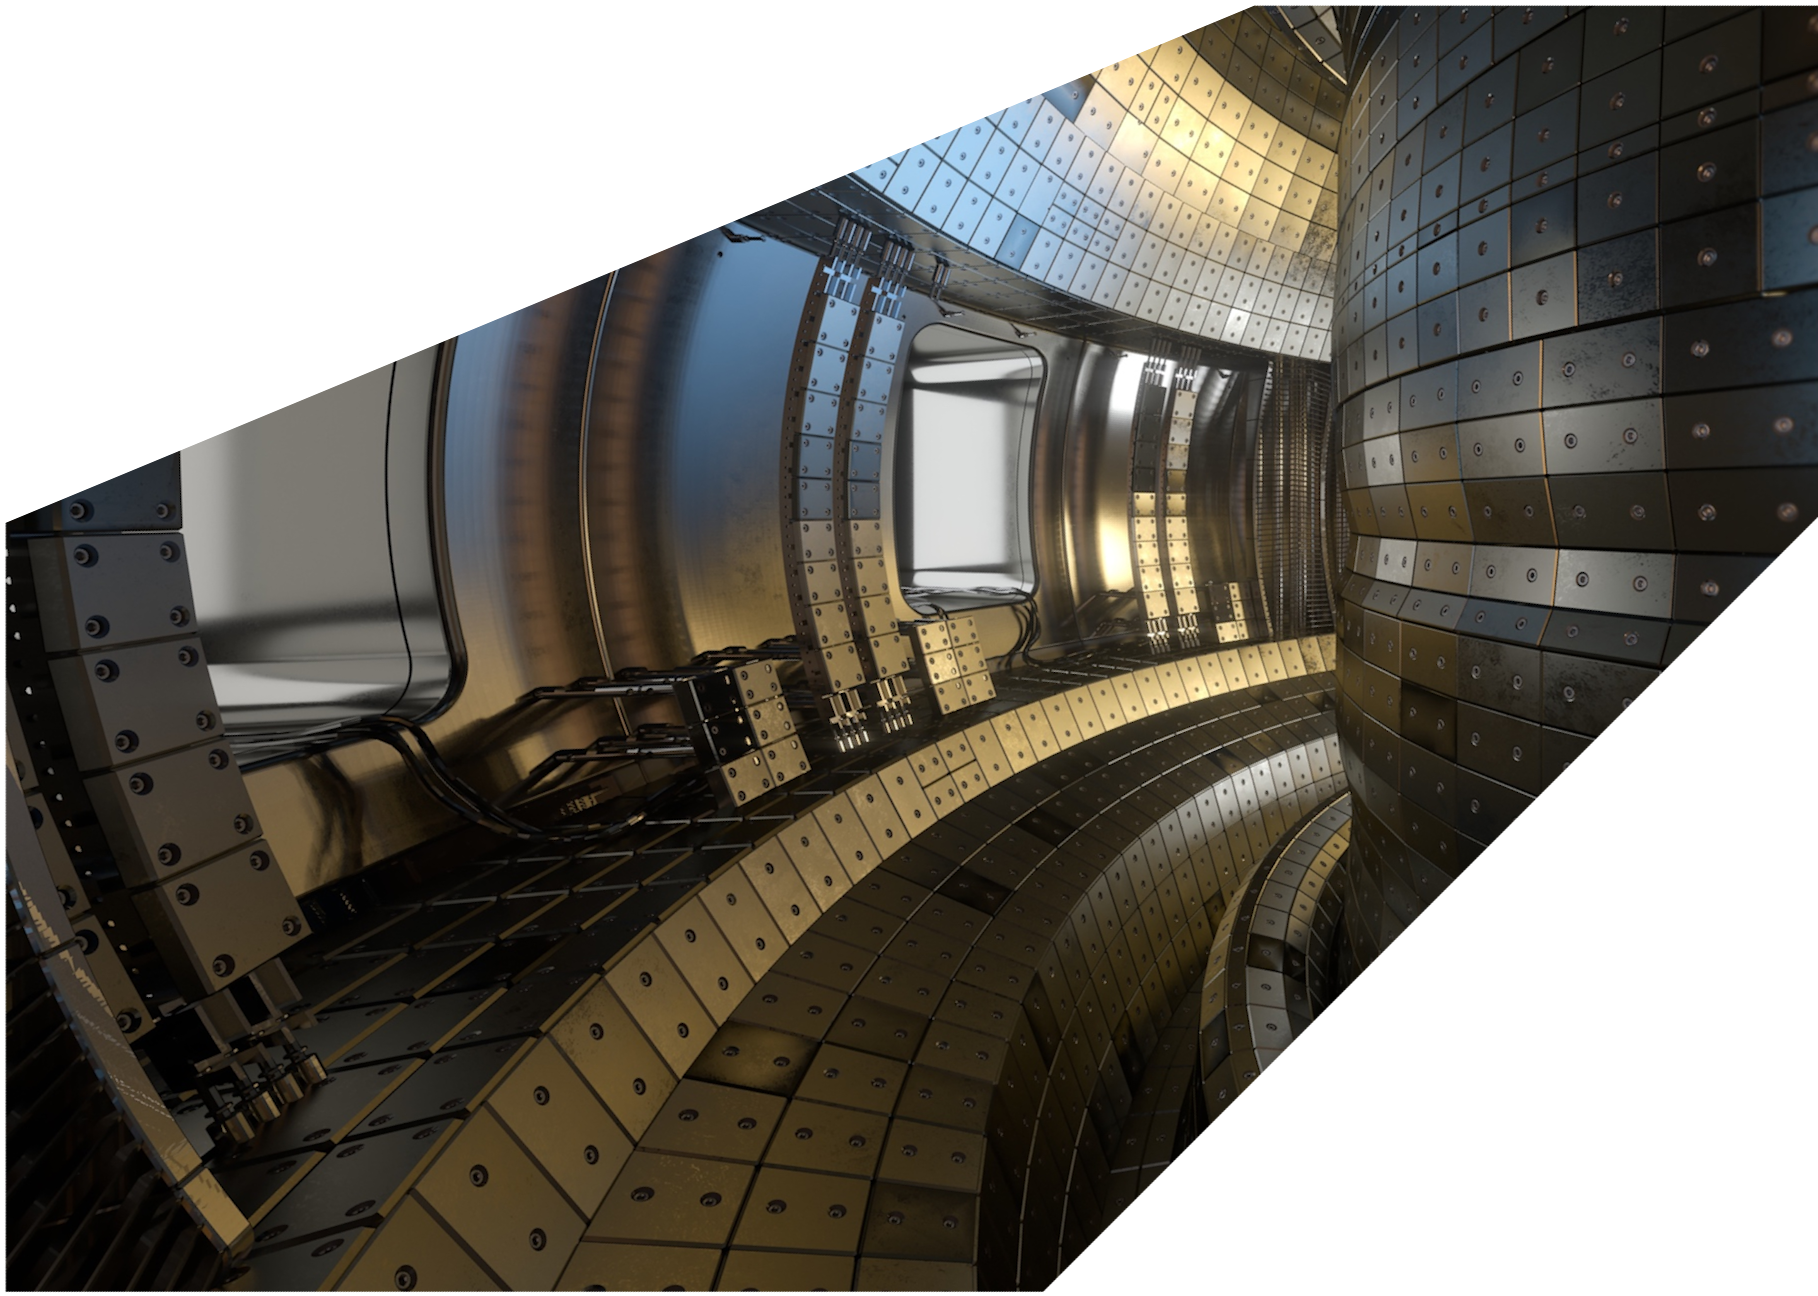
\includegraphics[width=0.9\textwidth]{../corpics/tokintcrop}}%<==omit
\end{titlepage}%<==omit

\hspace{-30mm}\begin{table}[h]
\sffamily
\begin{center}
\textbf{\textsf{UKAEA REFERENCE AND APPROVAL SHEET}}
\begin{tabular}{||p{5.7cm}|p{4.7cm}|p{5.0cm}||}
\hline
\hline
& Client Reference: &  \\
\hline
& UKAEA Reference: & \culhamshorttitle \\
& & \\
\hline
& Issue: & \culhamissueno \\
\hline
& Date: & \culhamdateb \\
\hline
\multicolumn{3}{||l||}{} \\
\multicolumn{3}{||l||}{Project Name: ExCALIBUR Fusion Modelling System} \\
\multicolumn{3}{||l||}{} \\
\hline
\end{tabular}
\begin{tabular}{||p{3.3cm}|p{4.6cm}|p{3.5cm}|p{3.6cm}||}
\hline
& Name and Department & Signature & Date \\
\hline
Prepared By: & \culhamauthora & N/A & \culhamdate \\
& \culhamauthor & N/A & \culhamdate \\
& & & \\
& BD & & \\
\hline
Reviewed By: & \culhamcontactname & 
\includegraphics[width=3.0cm]{../corpics/blanksign}& \culhamdatea \\
& & & \\
& Advanced Computing Dept. Manager & & \\
\hline
Approved By: & \culhamcontactname  & 
\includegraphics[width=3.0cm]{../corpics/blanksign} & \culhamdateb \\
& & & \\
& Advanced Computing Dept. Manager  & &\\
\hline
\hline
\end{tabular}
\end{center}
\end{table}


\clearpage
\input{body4}
\clearpage
\section*{Acknowledgement}\label{sec:ackn}
\emph{The support of the UK Meteorological Office and Strategic Priorities Fund is acknowledged.}


%\section*{References}
\bibliographystyle{unsrt}
\bibliography{../bib/new,../bib/waynes,../bib/misc,../bib/warv,../bib/neuts,../bib/reac,../bib/exc,../bib/active,../bib/dg1srt}

\end{document}
